
\section{Introduction}

%\subsection{Motivation and goals}

% stream processing for RT analytics
Real-time analytics are becoming increasingly prevalent in many businesses. 
Examples include Yahoo's Flurry~\cite{flurry},  
%\footnote{\url{https://developer.yahoo.com/flurry/docs/analytics/}},
the technology behind Mobile Developer Analytics, and Digits Yahoo Corporate-Wide dashboard for monitoring KPIs and traffic trends%at different granularities
~\cite{digits},
%\footnote{\url{https://digits3.yahoo.com}},
as well as Google's F1~\cite{Shute2013}, which powers its AdWords
%\footnote{\url{https://www.google.com/adwords/}}
business.
Such systems need to process massive data streams and answer queries about them in real-time.
% examples
A common query, for example, is estimating the number of \emph{unique elements} in a long stream, which 
can be used to count how many different users access a particular web page or application. 
A second example is a \emph{quantiles} estimator, which can be used, for example, to  answer questions like  \emph{what percentage of user sessions end within one minute?} or \emph{what is the median session time?}

% Sketches
In order to serve such queries, analytics engines use 
\emph{data sketches}, or \emph{sketches} for short. A sketch is essentially 
a succinct summary of a long stream. 
Sketches are built in a single pass over the stream via sampling or by applying a filter 
that retains a small subset  of the stream elements. 
%They are designed to take up a small memory footprint, since analytics engines 
%often keep tens or hundreds of thousands and sometimes even millions of 
%sketches in memory~\cite{Druid}.
% Sketches are fast
Due to the massive scale of the incoming data,   library functions producing sketches
are optimized to be extremely fast, often digesting millions of stream elements per second~\cite{sketchesLibrary}. 

%For example, the $\$ sketch in the Java Sketches Library \inred{add reference} 
%estimates the number of unique elements in a stream; it can process millions of stream 
%elements a second. 

 % Missing: r-w concurrency 
 Analytics engines need to answer real-time queries while  stream data continues to flow in.
 One way this is done 
today is by building sketches in epochs, and querying the sketch only after
 the epoch ends. An alternative approach is using locks to prevent concurrent access to a sketch.
 For example, in the Data Sketches Library~\cite{sketchesLibrary},  an 
attempt to query a sketch  while it is being updated  may encounter an inconsistent
intermediate state, leading to a gross estimation error. Therefore, applications like Druid~\cite{druid}
currently use sketches conservatively within a \emph{synchronized} block.
% and queries directed to a sketch must wait  for its construction to complete. 
Our first goal in this paper is to eliminate such waiting, and to allow queries to proceed 
concurrently with stream updates. 

% MIssing: w-w concurrency
In addition to the required concurrency among queries and updates,
it is also desirable to allow
concurrency among update threads in order to expedite the sketch building process on multi-core platforms. 
The common approach today is to build separate sketches from substreams, 
and then merge them via a dedicated union operation~\cite{multi-KMV}. 
In this approach, queries cannot be served before the final union completes. 
Our second goal is therefore to allow multiple threads to update a common, 
queryable sketch. The challenge is to do so without slowing down the update threads,
given that access to shared data requires  synchronization via costly memory fences 
and shared data updates can cause frequent invalidations in L1 caches, severely impacting performance. 
Figure~\ref{fig:lockBased} shows the throughput of two  popular
sequential sketch implementations from~\cite{sketchesLibrary} with
and without a lock. We see that 
the cost of acquiring a lock  is  high, since  sketches are
inherently fast structures.

\begin{figure}[t!]
    \centering
    \begin{subfigure}[t]{0.49\columnwidth}
       \centering
        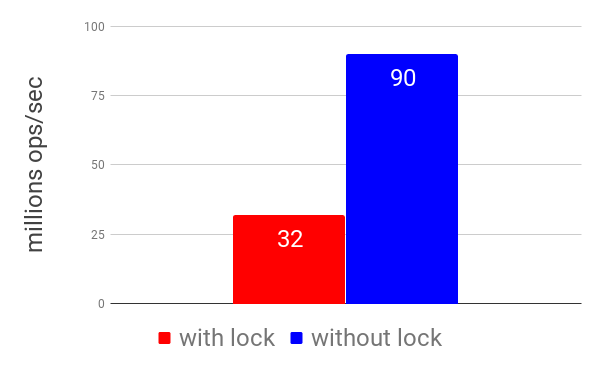
\includegraphics[width=1.5in]{images/seqTheta}
        \caption{$\Theta$ sketch}
        \label{fig:LockIsBadTheta}
    \end{subfigure}%
    \begin{subfigure}[t]{0.49\columnwidth}
        \centering
        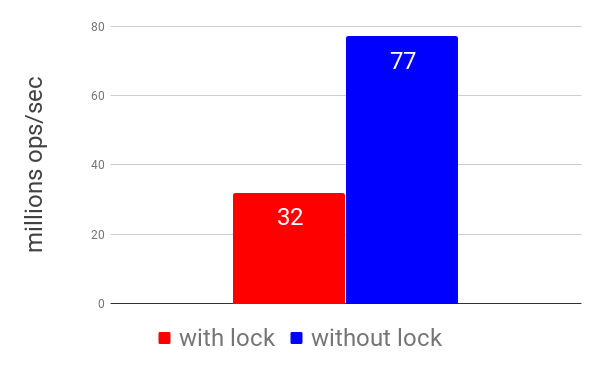
\includegraphics[width=1.5in]{images/seqQuantiles}
        \caption{Quantile sketch}
        \label{fig:LockIsBadQuantiles}
    \end{subfigure}
    \caption{Throughput of sequential sketch vs. lock-based sketch running a single write-only thread.}
    \label{fig:lockBased}
\end{figure}



% This paper
In this paper 
we present a general approach for building concurrent sketches that
constantly reflect all data processed by multiple update threads, 
and serve queries at any time. % during the stream processing. 
 % Basic idea for parallelizing
Our  approach employs multiple worker threads that buffer sketches of bounded-size substreams in thread-local memory, while a dedicated helper thread 
periodically \emph{propagates} these local buffers into a shared data structure via a union-like operation.
 Reducing data contention and the frequency of synchronization between the worker threads and the propagator is instrumental for achieving good performance. Queries are served from the shared data structure, and are carefully 
 designed to take its \emph{consistent snapshot} in case it is updated in parallel with them.

We implement our approach for two popular sketches in the Data Sketches Library -- $\Theta$~\cite{Theta},
which estimates the number of unique elements in a stream, and quantiles~\cite{quantiles}.
%worst-case error an adversarial scheduler can induce, 
Experiments show the algorithms scales almost linearly: with 28 threads, update throughput is an order of magnitude greater than with a single threads, while the 
read throughput is 3 orders of magnitude greater than that of a lock-based implementation.  


 
